\documentclass{article}

% Language setting
% Replace `english' with e.g. `spanish' to change the document language
\usepackage[english]{babel}

% Set page size and margins
% Replace `letterpaper' with `a4paper' for UK/EU standard size
\usepackage[a4paper,top=2cm,bottom=2cm,left=3cm,right=3cm,marginparwidth=1.75cm]{geometry}


\RequirePackage{multirow}  % 列合并需要的宏包
\RequirePackage{array}	   % 对齐相关的宏包
\RequirePackage{booktabs}  % 三线表宏包
\RequirePackage{tabularx}  % 自动平均分配列宽的宏包
\RequirePackage{longtable} % 跨页表格需要的宏包
\RequirePackage{tabu}      % 大表格需要的宏包
\RequirePackage{threeparttable} % 三段式表格,主要用于表格内引用
\usepackage{subcaption}
\usepackage{caption}

% Useful packages
\usepackage{pgf-pie}
\usepackage{geometry}
\usepackage{amsmath}
\usepackage{graphicx}
\usepackage[colorlinks=true, linkcolor=blue,backref=true]{hyperref}
\usepackage[hyperref=true,backref=true,style=ieee, backend=biber,isbn=true]{biblatex}
\addbibresource{refinfo.bib}
\usepackage{pgfplots}
\pgfplotsset{compat=1.18}

\title{Utilizing Generative AI for Personalized Learning in Computer Science Education}
\author{Baihan Deng,Daozheng Xue,Xiaoze Fan,Yumin Zhuang}

\begin{document}
\maketitle

\begin{abstract}
Your abstract.
\end{abstract}

\tableofcontents
\label{toc_contenttable}
\newpage

\section{INTRODUCTION}
\paragraph{}
Considering GenAI's huge effect in the future, it is very important to discuss how AI can help students appropriately; and those CS students who have been helped by GenAI can take part in GenAI's development in return, so it is also an interesting topic. In previous researches, we find that some studies focus on the practicality of AI-assisted programming and examine professional programmers' perspectives on it, like ``A Large-Scale Survey on the Usability of AI Programming Assistants: Successes and Challenges."\cite{liang-2023-LargeScaleSurveyUsability} and ``Expectation vs. Experience: Evaluating the Usability of Code Generation Tools Powered by Large Language Models"\cite{vaithilingam-2022-ExpectationVsExperience}.

\paragraph{}
Some studies focus on the general impact of generative AI on education, like ```Students' use of large language models in engineering education: A case study on technology acceptance, perceptions, efficacy, and detection chances"\cite{bernabei-2023-StudentsUseLarge} and ```With Great Power Comes Great Responsibility!': Student and Instructor Perspectives on the influence of LLMs on Undergraduate Engineering Education"\cite{joshi-2023-GreatPowerComes}.

\paragraph{}
Others pay attention to exploring AI-assisted computer education(``Beyond Traditional Teaching: Large Language Models as Simulated Teaching Assistants in Computer Science"\cite{liu-2024-TraditionalTeachingLarge}), exploring the possibility of AI teaching assistants from an educator's perspective(``Bob or Bot: Exploring ChatGPT's Answers to University Computer Science Assessment"\cite{richards-2024-BobBotExploring} and ``ChatGPT in the Classroom: An Analysis of Its Strengths and Weaknesses for Solving Undergraduate Computer Science Questions"\cite{joshi-2024-ChatGPTClassroomAnalysis}) or testing AI in answering CS-related questions, investigating the extent of students' trust in AI(``Trust in Generative AI among Students: An exploratory study"\cite{amoozadeh-2024-TrustGenerativeAI}).

\paragraph{}
In summary, the previous studies pay much attention to GenAI's effect on education generally, however, we do not find any study taking research on CS students specifically—a hard-to-begin major's students. As a group whose major is related to AI, it is hard to say whether these students' trust level on GenAI is same with other students'. Also, considering different learning content, it remains unknown whether the general study method(with GenAI) suits the CS student. So in this article, we'll discuss how does students and instructors trust GenAI and how to guide CS students to use GenAI to assist their personalized learning, in the hope of giving CS students some advise through our study.


\section{METHODOLOGY}
\paragraph{}
The methodology for this study is designed to evaluate the impact of generative AI (GenAI) tools on personalized learning within computer science (CS) education. To ensure a comprehensive understanding, the data collection and analysis approach integrates both quantitative and qualitative methods.

\subsection{Survey Design}
\paragraph{}
A structured questionnaire was developed to gather detailed insights from computer science students regarding their use and perceptions of generative AI tools. The questionnaire includes both closed and open-ended questions, addressing various aspects of GenAI usage in CS educational settings.

\paragraph{}
The survey questionnaire is divided into five parts:
\begin{itemize}
    \item \textbf{Understanding and Usage} This section includes questions about participants' understanding of GenAI and the frequency of its use in their learning. These questions categorize participants into users and non-users of GenAI.
    \item \textbf{Application and Acceptance} This section explores how participants use GenAI, including the specific aspects of their studies where they employ generative AI, their level of acceptance towards AI-assisted learning, and whether AI has enhanced their efficiency.
    \item \textbf{Trust} This section assesses the participants' trust in GenAI, using three targeted questions to address various levels of trust.
    \item \textbf{Concerns} This section addresses participants' concerns about GenAI, such as data privacy, security issues, and potential negative impacts on skill development.
    \item \textbf{Additional Opinions} This final part includes an open-ended question for participants to share any additional opinions on the use of GenAI in CS learning.
\end{itemize}

\paragraph{}
By structuring the survey in this manner, we aim to acquire a comprehensive understanding of participants' opinions on using GenAI in CS learning. Most of the questions are multiple-choice, with four options provided for frequency or degree measurements. For questions regarding reasons and aspects, multiple choices are available, along with an ``Other" option for additional inputs. This design facilitates quantitative analysis of the responses.






%  \begin{itemize}
%  \item Perceptions of students using GenAI(eg. ChatGPT, GitHub Copilot) in programming assignments.

% \item Challenges or barriers encountered when using GenAI as teaching assistant in Computer Science courses.

% \item Suggestions for integrating GenAI into CS curriculum and instructional practices.
% \end{itemize}

\section{RESULTS}
\paragraph{}
The survey questionnaire was distributed to computer science students at various levels of study, from undergraduate to graduate programs. A total of 101 valid responses were collected. Table \ref{table:response_distribution} lists the Distribution of Survey Responses by Academic Level.

\begin{table}[ht]
\centering
\captionsetup{labelfont={bf},textfont={bf}}
\caption{\label{table:response_distribution}\textbf{Distribution of Survey Responses by Academic Level}}
\begin{tabular}{>{\raggedright}p{4cm}rr}
\toprule
Student levels & Subtotal & Proportion \\
\midrule
Undergraduate Year 1 & 51 & 50.50\% \\
Undergraduate Year 2 & 18 & 17.82\% \\
Undergraduate Year 3 & 11 & 10.89\% \\
Undergraduate Year 4 & 5 & 4.95\% \\
Graduate & 16 & 15.84\% \\
\midrule
Total Valid Responses & \textbf{101} & \\
\bottomrule
\end{tabular}
\end{table}

\subsection{Students' knowledge about AI}
\paragraph{}
When asked about their level of understanding of generative AI such as ChatGPT, Claude, and Gemini, 42.57\% of respondents indicated they had a general understanding, while 47.52\% said they were familiar with these tools(Figure \ref{fig:understanding}). Only 9.9\% reported being unfamiliar with generative AI. This suggests that the majority of computer science students surveyed have at least a basic understanding of generative AI technologies, which may contribute to their willingness to adopt these tools in their learning process.
\begin{figure}[h!]
    \centering
    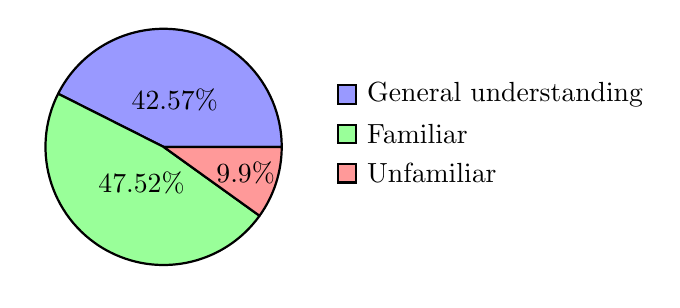
\begin{tikzpicture}
        \pie[
            text=legend,
            radius=1.5,
            color={blue!40, green!40, red!40}
        ]{
            42.57/General understanding,
            47.52/Familiar,
            9.9/Unfamiliar
        }
    \end{tikzpicture}
    \caption{Respondents' Level of Understanding of Generative AI}
    \label{fig:understanding}
\end{figure}
\subsection{Students' usage of AI}
\paragraph{}
The majority of respondents (65.35\%) reported using generative AI frequently in their studies(Figure \ref{fig:usage_frequency}), while 23.76\% used it occasionally. Only 4.95\% reported never using generative AI. The main purposes for using these tools (Figure \ref{fig:usage_purposes}) included assisting with programming (68.75\%), writing papers (87.5\%), and solving problems encountered in learning (80.21\%). These findings indicate that generative AI has become an integral part of many computer science students' learning strategies, with a wide range of applications across different aspects of their studies.
\begin{figure}
\centering
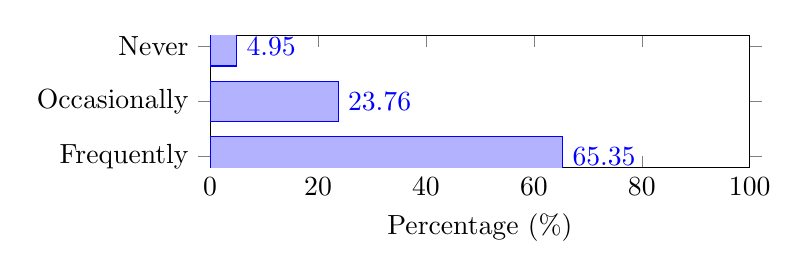
\begin{tikzpicture}
\begin{axis}[
    xbar,
    bar width=0.5cm,
    y=0.7cm,
    xmin=0,
    xmax=100,
    xlabel={Percentage (\%)},
    symbolic y coords={Frequently, Occasionally, Never},
    ytick=data,
    nodes near coords,
    nodes near coords align={horizontal},
    ]
\addplot coordinates {(65.35,Frequently) (23.76,Occasionally) (4.95,Never)};
\end{axis}
\end{tikzpicture}
\caption{Frequency of generative AI usage among respondents}
\label{fig:usage_frequency}
\end{figure}

\begin{figure}
\centering
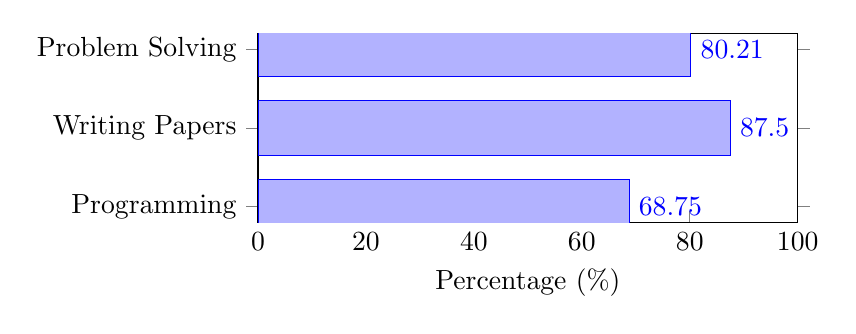
\begin{tikzpicture}
\begin{axis}[
    xbar,
    bar width=0.7cm,
    y=1cm,
    xmin=0,
    xmax=100,
    xlabel={Percentage (\%)},
    symbolic y coords={Programming, Writing Papers, Problem Solving},
    ytick=data,
    nodes near coords,
    nodes near coords align={horizontal},
    ]
\addplot coordinates {(68.75,Programming) (87.5,Writing Papers) (80.21,Problem Solving)};
\end{axis}
\end{tikzpicture}
\caption{Main purposes for using generative AI among respondents}
\label{fig:usage_purposes}
\end{figure}
\subsection{The role AI plays among students}
\paragraph{}
When asked about the helpfulness of generative AI in their learning, 45.54\% found it very helpful, and 37.62\% found it somewhat helpful. The main benefits reported were improved learning efficiency (82.18\%), expanded knowledge (49.5\%), enhanced programming skills (49.5\%), and others such as helping with creative inspiration (50.5\%) and providing learning resources (47.52\%). These results suggest that generative AI is playing a significant role in supporting and enhancing computer science students' learning experiences, with a majority of respondents recognizing its positive impact on various aspects of their academic development.
\subsubsection{Specific performance of AI in coding tasks}
\paragraph{}
Regarding the use of AI programming assistants like Copilot, 25.74\% of respondents reported using them frequently, while 26.73\% used them occasionally. When asked about the impact of these tools on their programming efficiency, 30.19\% reported a significant increase, and 45.28\% reported a moderate increase. This indicates that AI programming assistants are gaining popularity among computer science students and are perceived as valuable tools for boosting coding productivity.

\paragraph{}
In terms of the impact on code correctness, 64.15\% of respondents believed that AI helped improve the correctness of their code, while 26.42\% reported no noticeable impact. As for the impact on debugging efficiency, 43.56\% reported that AI helped improve their debugging efficiency, while 48.51\% reported no noticeable impact. These findings suggest that AI programming assistants have the potential to enhance code quality and streamline the debugging process for a significant portion of students, although the extent of their impact may vary depending on individual experiences and the specific tools used.

\subsection{Students’ level of trust in AI}
\subsubsection{The scale of their trust}
\paragraph{}
Regarding the correctness of AI's explanations of concepts(Figure \ref{fig:ai_trust}), 57.42\% of respondents believed in AI's abilities (22.77\% strongly believed, 34.65\% believed), while 34.65\% were neutral. For AI's reasoning abilities, 49.5\% believed in AI (14.85\% strongly believed, 34.65\% believed), and 36.63\% were neutral. As for AI's creative abilities, 48.51\% believed in AI (13.86\% strongly believed, 34.65\% believed), while 35.64\% were neutral. These results indicate that a substantial proportion of computer science students have a relatively high level of trust in generative AI's capabilities across different domains, although there is still a significant percentage who remain neutral or skeptical.
\begin{figure}[h!]
    \centering
    \begin{subfigure}{0.32\textwidth}
        \centering
        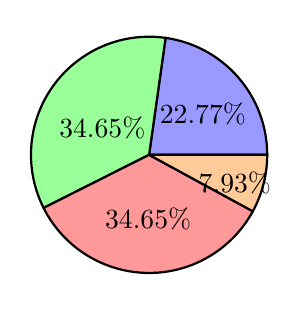
\begin{tikzpicture}
            \pie[
                text=inside,
                radius=1.5, % 半径为1.5厘米
                color={blue!40, green!40, red!40, orange!40}
            ]{
                22.77/,
                34.65/,
                34.65/,
                7.93/
            }
        \end{tikzpicture}
        \caption{Perception Abilities}
    \end{subfigure}
    \begin{subfigure}{0.32\textwidth}
        \centering
        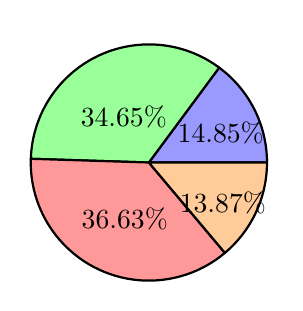
\begin{tikzpicture}
            \pie[
                text=inside,
                radius=1.5, % 半径为1.5厘米
                color={blue!40, green!40, red!40, orange!40}
            ]{
                14.85/,
                34.65/,
                36.63/,
                13.87/
            }
        \end{tikzpicture}
        \caption{Reasoning Abilities}
    \end{subfigure}
    \begin{subfigure}{0.32\textwidth}
        \centering
        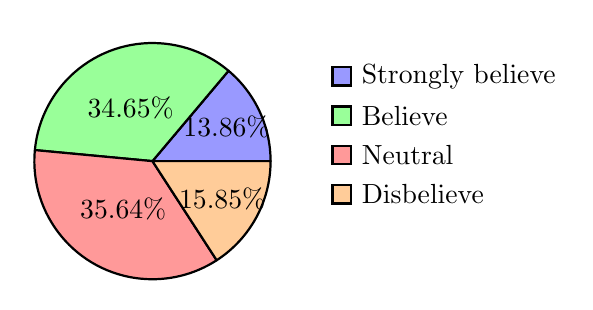
\begin{tikzpicture}
            \pie[
                text=legend,
                radius=1.5, % 半径为1.5厘米
                color={blue!40, green!40, red!40, orange!40}
            ]{
                13.86/Strongly believe,
                34.65/Believe,
                35.64/Neutral,
                15.85/Disbelieve
            }
        \end{tikzpicture}
        \caption{Creative Abilities}
    \end{subfigure}
    \caption{Respondents' Trust in Generative AI's Capabilities}
    \label{fig:ai_trust}
\end{figure}
\subsubsection{Why they hold that belief}
\paragraph{}
The reasons for students' trust or distrust in AI were not directly addressed in the survey. However, the frequent use of AI tools and the reported benefits suggest that positive experiences with AI contribute to students' trust. Additionally, the respondents' level of familiarity with generative AI technologies may also influence their trust, as those with a better understanding of AI's capabilities and limitations might have more informed opinions on its reliability.
\subsection{Other important information}
\paragraph{}
When asked about concerns regarding the use of generative AI, 37.62\% of respondents were worried about data privacy and security issues, while 52.48\% were not particularly concerned, and 9.9\% were not concerned at all. This suggests that while data privacy and security are important considerations for a significant portion of students, the majority do not view them as major barriers to using generative AI tools in their learning.

\paragraph{}
Regarding the potential negative impact of generative AI on skill development and employment prospects, 50.5\% of respondents believed it would not have a negative impact, while 12.87\% believed it would, and 36.63\% were unsure. The open-ended responses provided some insights into the reasons behind these beliefs. Some students expressed concerns that AI might replace certain job roles or lower the entry barrier, leading to increased competition. Others noted that AI could help automate low-level tasks, allowing students to focus on higher-level skills and adapt to the changing landscape of the computer science field.

\paragraph{}
These results provide a nuanced picture of computer science students' perceptions and experiences with generative AI in their learning. While the majority of respondents recognize the benefits and actively use these tools, there are still concerns and uncertainties that need to be addressed through further research, education, and guidance on the responsible and effective integration of AI in computer science education.

\section{DISCUSSION}
\subsection{How to guide CS students to use AI to assist their personalized learning}
\subsubsection{The Feature of CS Students}

\paragraph{}
According to the general curriculum requirements of computer science, We focus our attention on the following aspects:
\paragraph{}
Need of the knowledge from the wide range of fields.
The knowledge of the computer science has a significant difference from other major,
Which is different from other traditional major such as Physics and mathematics.  To traditional major A comprehensive knowledge framework is usually constructed, and students start their learning by understanding the construction of this knowledge framework and gradually progress through it. But to a new CS students, the language just like the basic rules, which cannot be Deductive reasoning by the existing knowledge. It is a system that is very rich and complex in content. And because of the dispersed characteristics of language, So the importance of the search engine is vast.
In that case , the effect of concise search is in need.
\paragraph{}
Practice of the programming and debug
Programming and debug are the basic skills of a CS students. They all need a students familiar with the programming language and the possible mistake. But as the programming is in need of high accuracy, some mirror mistake will cause a disaster result. Maybe the mistake is obvious by the AI, but the students could not find it in a short time. Then,  The debug will cost a lot of meaningless time.  Plus, the repeated programming will also spent a lot of energy.
\subsection{The Way of learning with AI.}
\paragraph{}
According to our research, AI has already play a important role in the CS students’ study .A great part of students often use GenAI to assist with their study (65.35 percentages),and almost every student has the experience to use GenAI(95.15 percentages).But when it comes to the programming, the rate declines rapidly. Only 25.74 percentages of students often use GenAI. The result reveals that the AI has widely used by CS students, but targeted applications of programming have not yet become widespread. So we will discuss some ways to use AI targeted for CS students.
\subsubsection{To get the information more efficient and targeted}
\paragraph{}
As we have discussed, The complex knowledge system is the feature of CS. While the traditional search engine is inefficient in front of the scattered knowledge, AI could efficiently retrieval and filtering. In fact, Expanding one's knowledge and providing learning resources is a common direction many students pursue when using AI.(49.5 percentages and 47.52percentages).
\paragraph{}
Additionally, CS often need the creative solutions to a specific problem, which is the weakness of traditional search engine. But students can ask to AI for some constructive suggestion, getting the inspire from the answer.

\subsubsection{Programming under the assistance of AI may be more friendly to beginners.}
\paragraph{}
As the programming and debug are the most time-consuming part of beginners learning, They could apply AI to their daily work.  According to our research, The majority of students agree that the AI could enhance their programming and debug efficiency. It could be a powerful tool for beginners to finish their works.But to a beginners, the most important things is how to provide their skills. Enhancing the efficiency but not becoming a obstacle to them could be a future learning direction.


\section{CONCLUSION}
\paragraph{}
In conclusion, our study focus on utilizing Generative AI for personalized learning in CS education,and through our study, we find out that it can benefit CS students a lot,as long as CS students use them in correct ways.
\paragraph{}
We find out that a large part of CS students know Generative AI and use it to help them complete tasks usually.While more than half of them believe in AI’s solving-problem ability, some of them do worry about data security.
\paragraph{}
Comparing with all college students, CS students show higher usage frequency and trust level about AI and lower worry level about information leakage.This may be because their major is more relevant to this area.Through our study, we have further improved CS students’ view about Generative AI and relative things which haven’t been studied specifically.
\paragraph{}
What can not be ignored is that limited by limited time, allocation and researchers,we only get about 100 answer sheets thus our discovery may have some degree of randomness.At the same time, we do not track students’learning life so we do not get data about AI’s real influence on CS students in the long term.
\paragraph{}
However, our study do get data about CS students’ opinion on Generative AI.And based on the data we collect, we recommand that CS students should use Generative AI more targeted,and do not worry about asking Generative AI to help you write, check or explain your code.At the same time, we also hope that Generative AI can further strengthen the security of data.



\newpage
\appendix
\section{REFERENCES}
\nocite{*}
\printbibliography[heading=none]
\end{document}